In this section, we will detail the algorithms discussed earlier.

First, let's review the seeding algorithm. We will quickly introduce the benefits of using the Burrows-Wheeler transform to build an index. This transformation is used in the FM-index.

The FM-index is a compressed representation for the reference genome. It is widely used thanks to its lightweight memory footprint, which is sub-linear with respect to the size of the data. Searching for a pattern in the compressed text is also sub-linear in time, which makes it ideal for seeding. When a seed is located, a chunk is taken from the genome around the seed to perform the alignment with the query sequence. This chunk should be larger than the query with which it shares a seed, since there could be gaps in the alignment. More details are available online~\cite{wiki:FMIndex}, but the following work does not rely on how FM-index works. 
%% You could detail the algorithm more, but who cares.

After seeding, we have to continue to align on both sides of the chain. For the extension, dynamic programming algorithms are used. They may be compute-intensive (and compute-bound), but they provide an optimal solution to the alignment problem. We could actually use them to compute the whole alignment but it is much more efficient to run smaller alignments as left and right extensions of the seed. They rely on computing a matrix of size $N \times M$, $N$ and $M$ being the length of the query and target sequences respectively. As shown on Figure~\ref{fig:dpmatrix}, we place the target sequence as a row, and the query as a column. Each cell is filled with a score depending on the north cell, the west cell, and the north-west cell, and the current bases to align. For the pair of bases, it corresponds to row and the column. For the sake of simplicity, let's assume that we only count matches with a score $\alpha > 0$, mismatches with a score $\beta < 0$, and a score for insertion and deletion $\gamma < 0$. We define the relation for the score $S_{i,j}$ on cell $i,j$ related to bases $a_i$ and $b_j$ with the formula~\ref{equ:dp}. In the Figure~\ref{fig:dpmatrix}, $\alpha = 2$ and $\beta = \gamma = -1$. More detailed information can be found in ~\cite{Aluru:2005:HCM:1121650}.

\begin{equation}
	S_{i,j} = max \left\{
	\begin{array}{llll}
		S_{i-1, j-1} + \alpha & \mbox{if} & a_i = b_j \\
		S_{i-1, j-1} + \beta & \mbox{if} & a_i \neq b_j \\
		S_{i, j-1} + \gamma \\
		S_{i-1, j} + \gamma\\
		 \\
	\end{array}
	\right.
	\label{equ:dp}
\end{equation}



\begin{figure}[ht!]
	\centering
	\begin{subfigure}[t]{0.5\textwidth}
		\centering
		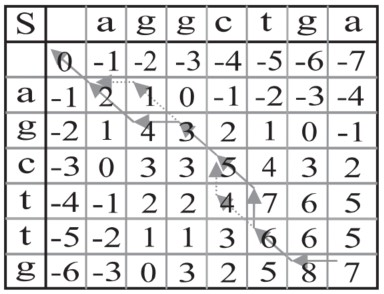
\includegraphics[height=0.5\textwidth]{global_align}
		\caption{Global alignment}
		\label{fig:global_align}
	\end{subfigure}%
	~ 
	\begin{subfigure}[t]{0.5\textwidth}
		\centering
		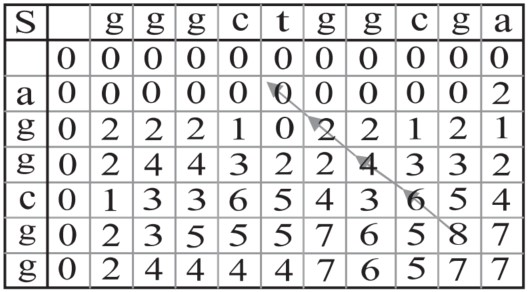
\includegraphics[height=0.5\textwidth]{local_align}
		\caption{Local alignment}
		\label{fig:local_align}
	\end{subfigure}
	\caption{Dyanmic programming alignments (from ~\cite{Aluru:2005:HCM:1121650}) }
	\label{fig:dpmatrix}
\end{figure}



Among dynamic programming (DP) algorithms, we can cite main techniques:

\begin{itemize}
	\item Needleman-Wunsch~\cite{NeedlemanWunsch:method}, or \emph{global} alignment: it tries to match the whole sequences. The results contains both sequences completely, as Figure~\ref{fig:global_align} shows, with the alignment path traversing the matrix. Mismatches on ends causes a penalty, as shows the negative scores on the edges;
	\item Smith-Waterman~\cite{SmithWaterman:identification}, or \emph{local} alignment: it aligns two sequences but only looks for the maximal score, which reports the best alignment there is. On Figure~\ref{fig:local_align}, one can see we select the best score, the score is initialised at 0 and stays positive;
	\item A mix of the two, \emph{semi-global}~\cite{Durand:course-genomics} alignment, that performs a global alignment but allows to skip both ends of the query sequence. In practical, semi-global is often used instead of global;
	\item BLAST~\cite{Altschul:BLAST}-like extension: it performs two alignments on both ends of the seed instead of aligning the sequences entirely. If first makes a local alignment on the left side, starting with a non-zero score, but taking the seed score instead. Then it makes a local alignment on the right side, starting as initial score the previous computed score (taking the seed and left alignment). This splits the alignment problem in two, which makes it much faster. This is the technique used in seed-extension.
\end{itemize}

The pseudocode for local alignment is presented in Algorithm~\ref{algo:local}. It computes the whole dynamic programming matrix $S$ with the equation~\ref{equ:dp} showed above. There are small difference between global, local and semi-global alignments in the initialisation step, the computing formula, and how the final score is obtained from the matrix. For the local alignment, which is the one we will use in the rest of the thesis, initialisation is done with a score of zero along both north and west edges of the matrix. This means that no penalty is made on the ends of both sequences. Second, in the computing formula showed in equation~\ref{equ:dp}, the score can actually go negative if a lot of mismatches occur. We do not want this behaviour with local alignment, meaning that there is no penalty if an area is not aligned (the alignment can occur later on in the sequence). In the Algorithm~\ref{algo:local}, this is shown by taking the maximum of the computed score with 0. Finally, in local alignment, we want the best possible score without constraints on the end of the alignment, so we simply take the maximum value in the dynamic programming matrix as the end position of the alignment.

\begin{algorithm}[h!]
	\caption{Dynamic programming matrix computation algorithm}
	\label{algo:local}
	\begin{algorithmic}[1] % The number tells where the line numbering should start
		\Procedure{Compute the dynamic programming matrix, local alignment}{$query\_string$, $target\_string$, $query\_length$, $target\_length$} \Comment{}
		

		\State \emph{Initialise score}
		\For{i from -1 to $query\_length$}
			\State $S_{i, -1} \leftarrow 0$
		\EndFor	
				
		\For{j from -1 to $target\_length$}
			\State $S_{-1, j} \leftarrow 0$	
		\EndFor
		
		\State \emph{compute S matrix}
		\For{ (i from $0$ to $query\_length - 1$}
			\For {j from $0$ to $target\_length - 1$}
			
				\State Read base $query\_base_i$ in $query\_string$
				\State Read base $target\_base_j$ in $target\_string$ 	
				\State $ 	S_{i,j} \leftarrow max \left\{
				\begin{array}{llll}
				S_{i-1, j-1} + \alpha & \mbox{if} & query\_base_i = target\_base_j \\
				S_{i-1, j-1} + \beta & \mbox{if} & query\_base_i \neq target\_base_j \\
				S_{i, j-1} + \gamma \\
				S_{i-1, j} + \gamma\\
				0 \\
				\end{array}
				\right. $
				
			\EndFor
			
		\EndFor
		
		\State Find $i_{max}$ and $j_{max}$ for which $S_{i_{max}, j_{max}} = max(S_{i,j})$
		\State $score \leftarrow S_{i_{max}, j_{max}}$
		\State $end\_position\_query \leftarrow i_{max}$
		\State $end\_position\_target \leftarrow j_{max}$
		
		\EndProcedure
		
	\end{algorithmic}
\end{algorithm}

On these algorithms, several optimisation can be added to speed them up. Depending on the technology at hand, one can use Single Instruction Multiple Data (SIMD) to compute several cells of the dynamic programming matrix at once. Another optimisation called \emph{z-dropoff} is interrupting the calculation of a row when the score drops sharply. Finally, it can be noticed that the north-east and south-west corners of the dynamic programming matrix are often useless to compute, since reaching these cells would mean that the alignment is containing a huge gap (and hence has a mediocre score). One can simply avoid to compute them, resulting in only calculating a band around the diagonal, hence calling this technique banded dynamic programming.
